\documentclass{assignment}

\course{ECO 120-04}
\name{Lucas Reddinger}
\date{Friday 23 September 2022}
\doctitle{Assignment 3: Demand}

\begin{document}
\RaggedRight

\beginassignment{}

\emph{Due Wednesday 28 September.} Please submit hardcopy at the beginning of class (11:00 a.m.), or if you prefer, under the door of Wimberly Hall 339C by 10:50 a.m.

\section*{Gas station labor}

You operate a gas station. Your employees could produce coffee for sale by brewing each pot manually; this takes 40 hours of work per week. Your employees could use a super-automatic coffee machine that only requires minimal attention of 10 hours of work per week. Or you could simply not sell coffee.

Suppose that if market wage rate $w\geq10$, you decide selling coffee is too expensive, so you do not sell coffee whatsoever. If $7 \leq w < 10$, you purchase and use a super-automatic coffee maker. If $w < 7$, you ask your employees to brew pots of coffee individually.

\begin{enumerate}

\item Please graph your company's demand curve for \emph{hours of coffee-making labor per week}. Label the horizontal axis with $L$ (hours of labor), using a range from 0 to 200. Label the vertical axis with $w$ (dollars per hour), using a range from 0 to 20. Please label your demand curve as $D_{\text{coffee }L}(w)$.

\begin{center}
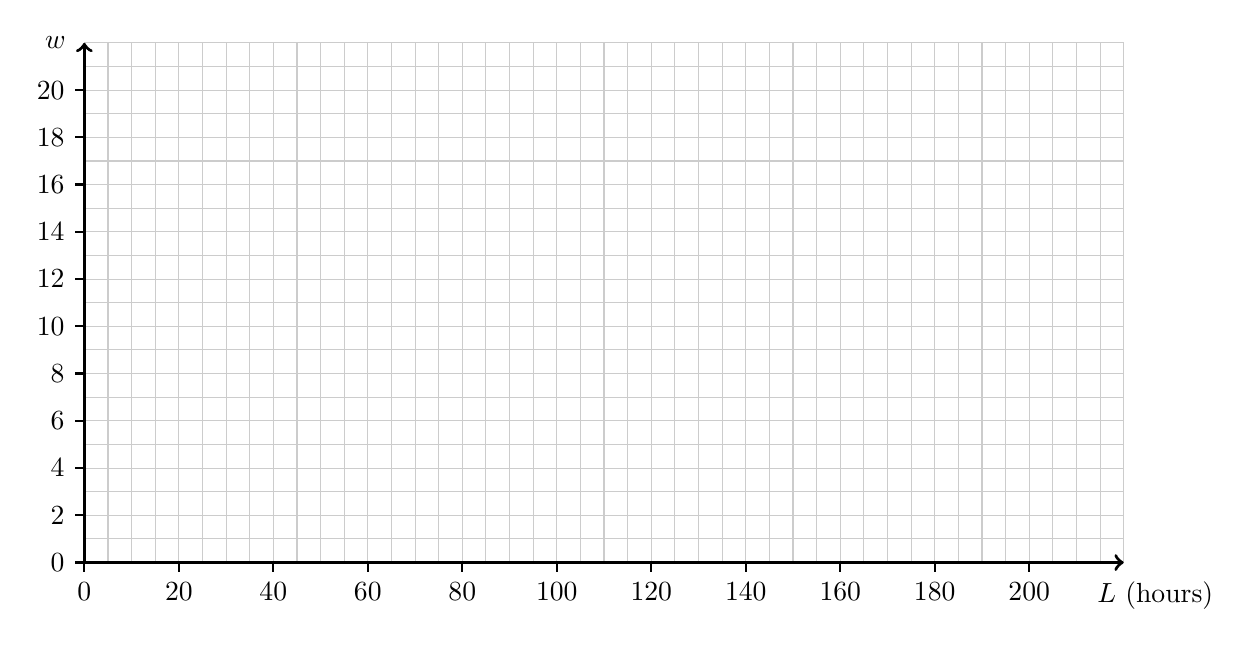
\begin{tikzpicture}[x=2mm,y=10mm,scale=0.3]
\draw[thin, black!20!white] (0,0) grid (220,22);
\foreach \i in {0,20,40,...,200}{\draw[thick] (\i,0mm) -- + (0,-4mm) node[below] {\i};}
\foreach \i in {0,2,4,...,20}{\draw[thick] (0mm,\i) -- + (-4mm,0) node[ left] {\i};}
\draw[very thick,->] (0,0) -- (0,22) node[left,xshift=-1mm] {$w$};
\draw[very thick,->] (0,0) -- (220, 0) node[below,xshift=4mm,yshift=-1mm] {$L$ (hours)};
\end{tikzpicture}
\end{center}

\clearpage

\item Of course, your gas station needs employees to work many other aspects of the station. You need 60 hours of labor per week for cashier work, and you're willing to pay over \$20 per hour for this work. Please draw this as a separate curve on the same graph; label this new curve $D_{\text{cashier }L}(w)$.

\item On the same graph, please construct a demand curve for the total labor you want to hire $D_{\text{total }L}(w)$ at any given wage $w$. Note that $D_{\text{total }L}(w) = D_{\text{coffee }L}(w) + D_{\text{cashier }L}(w)$.

\item Summer arrives and demand for your services doubles. To accommodate this demand, you can exactly double your output by doubling your factor inputs. That is, if you double the amount of labor you hire, you can double the service you provide. Mathematically, $D_{\text{summer total }L}(w)=2 \times D_{\text{total }L}(w)$. Please add to your graph a curve labeled $D_{\text{summer total }L}(w)$ to represent your total summer labor demand.

\item Suppose it's summer and the market wage rate is $w=8$. Mark this point on the demand curve $D_{\text{summer total }L}(w)$ as $E$. How much labor do you hire? Do you sell coffee, and if so, using what method of production?

\vfill

\item Suppose it's summer and the market wage rate is $w=5$. Mark this point on the demand curve $D_{\text{summer total }L}(w)$ as $F$. How much labor do you hire? Do you sell coffee, and if so, using what method of production?

\vfill

\item Suddenly, many workers have exited the labor force, so market wages have increased---now $10<w<20$. Consider how this might affect your demand for summer labor, $D_{\text{summer total }L}(w)$. Does the curve shift? Depict such an example on your graph, label it $G$, and describe it below.

\vfill

\end{enumerate}
\end{document}
